\documentclass[1pt]{elsarticle}

\usepackage{lineno,hyperref}
\usepackage{latexsym,amsthm,amsmath,xcolor,graphicx, amssymb, color,hyperref,booktabs,mathrsfs}

%\modulolinenumbers[5]

\usepackage{geometry}
 \geometry{
 letterpaper,
 total={8.5in,11in},
 left=.75in,
 right=.75in,
 top=.75in,
 bottom=.75in,
 }

\journal{}

% Macros
\renewcommand{\vec}[1]{{\mathchoice
                     {\mbox{\boldmath$\displaystyle{#1}$}}
                     {\mbox{\boldmath$\textstyle{#1}$}}
                     {\mbox{\boldmath$\scriptstyle{#1}$}}
                     {\mbox{\boldmath$\scriptscriptstyle{#1}$}}}}
\newcommand{\norm}[1]{\left\| {#1} \right\|}
\newcommand{\D}{\mathcal{D}}
\newcommand{\R}{\mathbb{R}}
\newcommand{\C}{\mathbb{C}}
\newcommand{\N}{\mathbb{N}}
\newcommand{\grad}{\nabla}
\newcommand{\hessian}{\nabla^2}
\newcommand{\V}{\mathscr{V}}
\renewcommand{\S}{\mathbb{S}}
\newcommand{\ST}{\mathbb{S}^{\text{tot}}}
\newcommand{\ip}[2]{\langle{#1}, {#2}\rangle}
\newcommand{\tp}{{\!\mathsf{T}}}
\newcommand{\mat}[1]{\mathbf{{#1}}}
\newcommand{\Np}{{N_\text{p}}}
\newcommand{\E}[1]{\mathrm{E}\left\{{#1} \right\}}

\newtheorem{theorem}{Theorem}[section]

%%%%%%%%%%%%%%%%%%%%%%%
%% Elsevier bibliography styles
%%%%%%%%%%%%%%%%%%%%%%%
%% To change the style, put a % in front of the second line of the current style and
%% remove the % from the second line of the style you would like to use.
%%%%%%%%%%%%%%%%%%%%%%%

%% Numbered
%\bibliographystyle{model1-num-names}

%% Numbered without titles
%\bibliographystyle{model1a-num-names}

%% Harvard
%\bibliographystyle{model2-names.bst}\biboptions{authoryear}

%% Vancouver numbered
%\usepackage{numcompress}\bibliographystyle{model3-num-names}

%% Vancouver name/year
%\usepackage{numcompress}\bibliographystyle{model4-names}\biboptions{authoryear}

%% APA style
%\bibliographystyle{model5-names}\biboptions{authoryear}

%% AMA style
%\usepackage{numcompress}\bibliographystyle{model6-num-names}

%% `Elsevier LaTeX' style
\bibliographystyle{elsarticle-num}
%%%%%%%%%%%%%%%%%%%%%%%

\begin{document}

\begin{frontmatter}

\title{Efficient UQ and sensitivity analysis for chemical systems using active 
subspaces}

%% Group authors per affiliation:
\author{Manav Vohra, Alen Alexanderian, Hayley Guy, Sankaran Mahadevan}
\address{Vanderbilt, NCSU}

%% or include affiliations in footnotes:
%\author[mymainaddress,mysecondaryaddress]{Elsevier Inc}
%\ead[url]{www.elsevier.com}

%\author[mysecondaryaddress]{Global Customer Service\corref{mycorrespondingauthor}}
%\cortext[mycorrespondingauthor]{Corresponding author}
%\ead{support@elsevier.com}

%\address[mymainaddress]{1600 John F Kennedy Boulevard, Philadelphia}
%\address[mysecondaryaddress]{360 Park Avenue South, New York}

\begin{abstract}
Insert abstract here.
\end{abstract}

\begin{keyword}
\texttt{elsarticle.cls}\sep \LaTeX\sep Elsevier \sep template
\MSC[2010] 00-01\sep  99-00
\end{keyword}

\end{frontmatter}

%\linenumbers

\section{Introduction}
Insert introduction here.

\section{Active subspaces and activity scores}
For $f: \Omega \to \R$, we consider the DGSMs~\cite{SobolKucherenko09},
\[
    \nu_j(f) := \E{\left(\frac{\partial f}{\partial\xi_j}\right)^2} =
                  \int_\Omega 
                  \left(\frac{\partial f}{\partial\xi_j}\right)^2
                  \pi(\vec{\xi})d\vec{\xi}, \quad j = 1, \ldots, \Np.   
\]
Here $\pi$ is the joint PDF of $\xi$. 
Let $\mat{C} = \E{\nabla f \nabla f^T}$.
We define the activity scores~\cite{Diaz16}
\[
   \alpha_j(f; r) =  \sum_{k=1}^r \lambda_k \ip{\vec{e}_j}{\vec{u}_k}^2,
   \quad j = 1, \ldots, \Np, \quad r \leq \Np.
\]
\begin{theorem}
Consider the spectral decomposition of $\mat{C}$, given by  
$\mat{C} = \sum_{k=1}^\Np \lambda_k \vec{u}_k \vec{u}_k^T$.
We have,
\begin{enumerate}
\item $\nu_j(f) = \sum_{k=1}^\Np \lambda_k \ip{\vec{e}_j}{\vec{u}_k}^2$.
\item $\alpha_j(f; r) \leq \nu_j(f) \leq \alpha_j(f; r) + \lambda_{r+1}$, 
for $j=1, \ldots, \Np$.
\end{enumerate}
\end{theorem} 

The utility of this result is realized in 
problems with 
high-dimensional parameter spaces in which 
the eigenvalues $\lambda_j$ decay rapidly to zero; in 
such cases, this result implies that  $\nu_j(f) \approx \alpha_j(f; r)$,
where $r$ is the \emph{numerical rank} of $\mat{C}$.  This will be especially
effective if there is a large gap in the eigenvalues.  


\section*{References}

\bibliography{mybibfile}

\begin{figure}[htbp]
 \begin{center}
  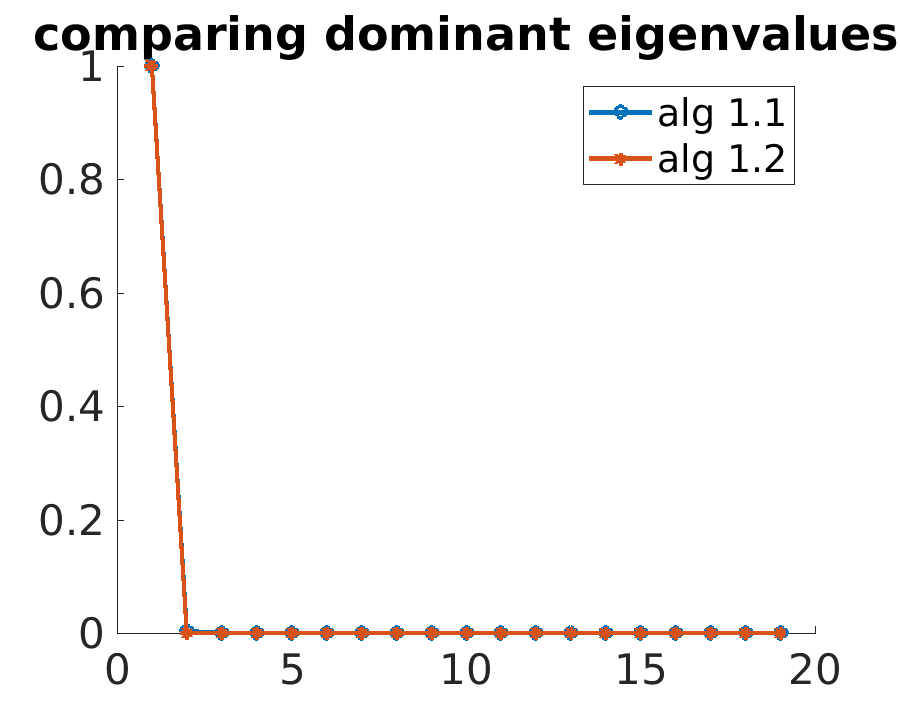
\includegraphics[width=0.44\textwidth]{./Figures/comp_eig}
\hspace{1mm}
  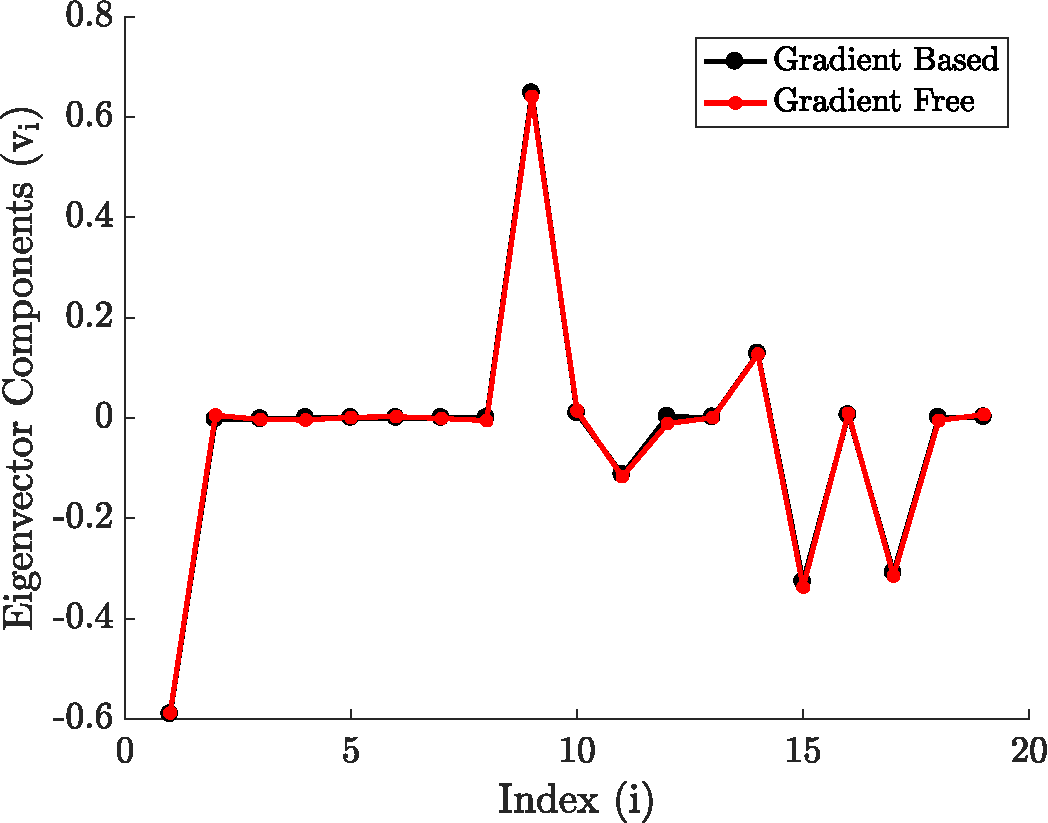
\includegraphics[width=0.48\textwidth]{./Figures/comp_eigv}
  \\ \vspace{5mm}
  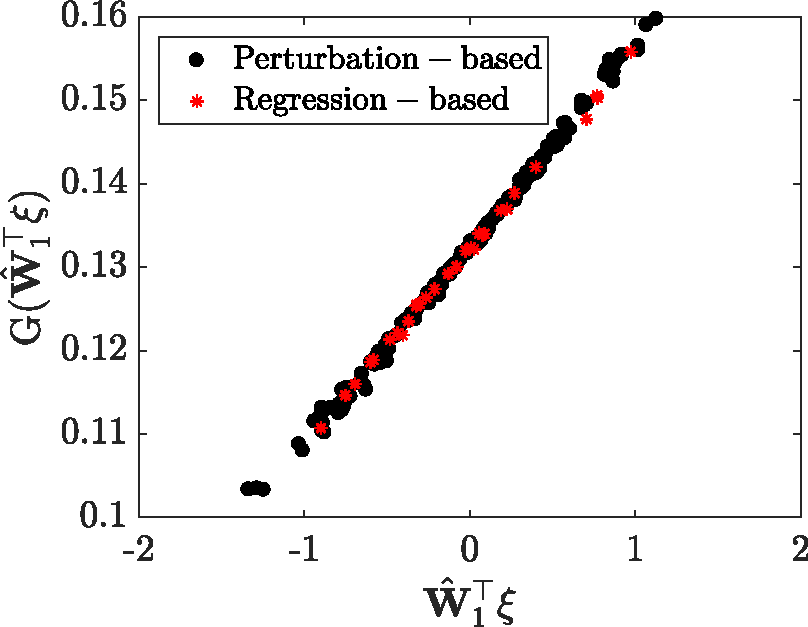
\includegraphics[width=0.44\textwidth]{./Figures/comp_ssp}
\hspace{1mm}
  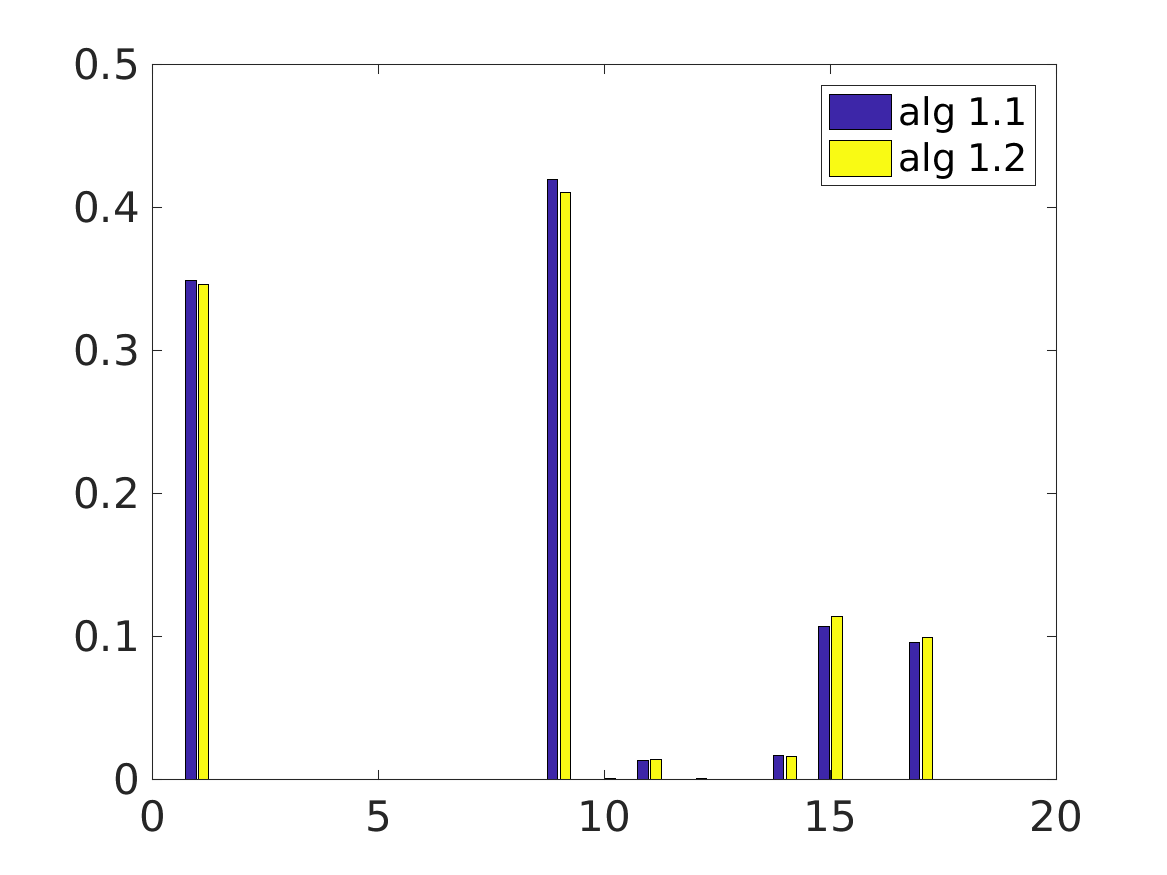
\includegraphics[width=0.48\textwidth]{./Figures/comp_as}
\end{center}
\end{figure}


\end{document}
